% ★★ 中档
\newcommand{\qConicHardHyperbolaMidpointStem}{
已知双曲线 $C: x^2 - \frac{y^2}{2} = 1$．过点 $M(0, 1)$ 的直线 $l: y = kx + 1$ 与双曲线 $C$ 交于不同的两点 $A, B$．
(1) 求斜率 $k$ 的取值范围；
(2) 设弦 $AB$ 的中点为 $N$，若 $\vec{OM} \cdot \vec{ON} = 2$，求直线 $l$ 的方程．
}
\newcommand{\qConicHardHyperbolaMidpointFigure}{
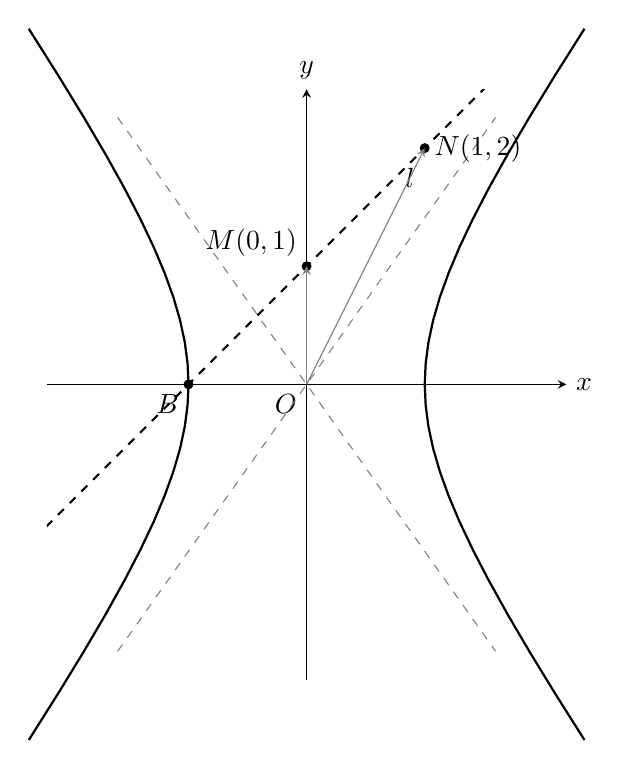
\begin{tikzpicture}[scale=1.5, >=stealth]
  % Axes
  \draw[->] (-2.2,0) -- (2.2,0) node[right] {$x$};
  \draw[->] (0,-2.5) -- (0,2.5) node[above] {$y$};
  \node[below left] at (0,0) {$O$};
  
  % Hyperbola
  \draw[thick, domain=-1.5:1.5] plot ({cosh(\x)}, {1.414*sinh(\x)});
  \draw[thick, domain=-1.5:1.5] plot ({-cosh(\x)}, {1.414*sinh(\x)});
  
  % Asymptotes
  \draw[dashed, gray, thin] (-1.6, -2.26) -- (1.6, 2.26);
  \draw[dashed, gray, thin] (-1.6, 2.26) -- (1.6, -2.26);
  
  % Point M(0, 1)
  \coordinate (M) at (0, 1.0);
  \fill (M) circle (1.2pt) node[above left] {$M(0,1)$};
  
  % Line l: y = x + 1 (intersects hyperbola at A(3,4) and B(-1,0))
  \coordinate (A) at (3.0, 4.0); % Out of bounds of plot, so let's clip
  \coordinate (B) at (-1.0, 0);
  \fill (B) circle (1.2pt) node[below left] {$B$};
  
  % Midpoint N(1, 2)
  \coordinate (N) at (1.0, 2.0);
  \fill (N) circle (1.2pt) node[right] {$N(1,2)$};
  
  % Draw line l clipped
  \begin{scope}
    \clip (-2.2, -2.5) rectangle (2.2, 2.5);
    \draw[thick, dashed] (-3.0, -2.0) -- (2.0, 3.0) node[right, near end] {$l$};
    \fill (1.8, 2.8) circle (1.2pt) node[above left] {$A$};
  \end{scope}
  
  % Vectors
  \draw[->, thin, gray] (0,0) -- (M);
  \draw[->, thin, gray] (0,0) -- (N);
\end{tikzpicture}
}
\newcommand{\qConicHardHyperbolaMidpointAnswer}{
(1) $k \in (-\sqrt{3}, -\sqrt{2}) \cup (-\sqrt{2}, \sqrt{2}) \cup (\sqrt{2}, \sqrt{3})$；\\
(2) 直线 $l$ 的方程为 $y = x + 1$ 或 $y = -x + 1$．
}
\newcommand{\qConicHardHyperbolaMidpointSolution}{
\begin{proof*}
(1) 直线 $l: y = kx + 1 \implies kx - y + 1 = 0$，对应硬解系数为 $A=k, B=-1, C=1$．\\
双曲线 $C: x^2 - \frac{y^2}{2} = 1 \implies \frac{x^2}{1} - \frac{y^2}{2} = 1$，对应参数为 $a^2=1, b^2=2$（注意双曲线中半轴平方为 $b^2 \to -b^2$）．\\
此时统一分母为 $D = A^2a^2 - B^2b^2 = k^2(1) - (-1)^2(2) = k^2 - 2$．\\
联立直线与双曲线方程，消去 $y$ 整理为：
\[
(2 - k^2)x^2 - 2kx - 3 = 0
\]
因为直线与双曲线交于不同的两点，根据双曲线硬解定理判定，分母 $D \neq 0$（直线不与渐近线平行）且 $C^2 > D$（相交判别式大于零）：
\[
\begin{cases}
2 - k^2 \neq 0 \\
1 > k^2 - 2 \implies k^2 < 3
\end{cases}
\]
解得：$k^2 \neq 2$ 且 $k^2 < 3$．\\
综上所述，斜率 $k$ 的取值范围为 $(-\sqrt{3}, -\sqrt{2}) \cup (-\sqrt{2}, \sqrt{2}) \cup (\sqrt{2}, \sqrt{3})$．\\

(2) 设 $A(x_1, y_1), B(x_2, y_2)$，由 (1) 的一元二次方程，中点 $N$ 的横坐标可以直接应用硬解公式得到：
\[
x_N = \frac{x_1 + x_2}{2} = -\frac{ACa^2}{D} = -\frac{k}{k^2-2} = \frac{k}{2 - k^2}
\]
因为中点 $N$ 在直线 $y = kx + 1$ 上，我们可以直接利用直线的点线共存关系求出其纵坐标，避免了使用纵坐标韦达定理并进行通分化简的繁重代数工作：
\[
y_N = k x_N + 1 = k\left(\frac{k}{2 - k^2}\right) + 1 = \frac{2}{2 - k^2}
\]
由点 $M(0, 1)$ 可知 $\vec{OM} = (0, 1)$，而 $\vec{ON} = (x_N, y_N)$，则：
\[
\vec{OM} \cdot \vec{ON} = 0 \cdot x_N + 1 \cdot y_N = y_N = \frac{2}{2 - k^2}
\]
因为 $\vec{OM} \cdot \vec{ON} = 2$，所以：
\[
\frac{2}{2 - k^2} = 2 \implies 2 - k^2 = 1 \implies k^2 = 1 \implies k = \pm 1
\]
经检验，$k = \pm 1$ 满足 $k^2 < 3$ 且 $k^2 \neq 2$，符合题意．\\
所以直线 $l$ 的方程为 $y = x + 1$ 或 $y = -x + 1$．
\end{proof*}
}
\newcommand{\qConicHardHyperbolaMidpointDiagnosis}{
\errortag{渐近线平行漏讨论} 很多学生在求 $k$ 范围时常常忘记限制 $2 - k^2 \neq 0$（即直线不能与双曲线渐近线平行），导致在求取值范围时出错。\\
\errortag{中点坐标消元错误} 在计算 $y_N$ 时，很多学生习惯用 $y_N = \frac{y_1+y_2}{2}$ 并用 $y$ 的韦达定理计算，这不仅繁琐，且容易算错负号。直接利用中点 $N$ 在直线 $l$ 上代入 $y_N = k x_N + 1$ 是一种极简的代数化简技巧。
}
